\documentclass{beamer}

\usepackage{tikz}
\usetikzlibrary{shapes.geometric, arrows, matrix, positioning, calc}

% Title and author information
\title{Introduction to Attention Mechanism in LLMs}
\subtitle{"Attention is all you need"}
\institute{Yanshan University}
\author{SkyRain}
\date{\today}
\setbeamertemplate{footline}[frame number]

\begin{document}

% Title slide
\begin{frame}
    \titlepage
\end{frame}

% Table of contents
\begin{frame}{Outline}
    \tableofcontents
\end{frame}

% Section 1
\section{Introduction about Attention Mechanism}
\begin{frame}{Introduction about Attention Mechanism}
    \begin{itemize}
        \item Attention mechanism is a key component of LLMs
        \item It allows the model to focus on different parts of the input
        \item Helps in understanding context and relationships
    \end{itemize}
    \begin{block}{Why Attention?}
        \begin{itemize}
            \item Traditional models struggled with long-range dependencies
            \item Attention mechanism overcomes this limitation
            \item Enables parallel processing of input data
        \end{itemize}
    \end{block}
\end{frame}

\begin{frame}{Compare with traditional models}
    \begin{block}{Traditional Models}
        \begin{itemize}
            \item RNNs and LSTMs
            \item Sequential processing
            \item Difficulty in capturing long-range dependencies
        \end{itemize}
    \end{block}
    \begin{block}{Attention Mechanism}
        \begin{itemize}
            \item Processes all tokens simultaneously
            \item Captures relationships between all tokens
            \item More efficient and effective for long sequences
        \end{itemize}
    \end{block}
\end{frame}

% Section 2
\section{Learning Attention Mechanism}
\begin{frame}{Key Concept}
    \begin{block}{LLM process numbers}
        \begin{center}
            % todo: replace vectorize, llm, decode with real numbers
            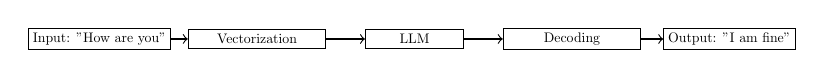
\begin{tikzpicture}[node distance=1.5cm, scale=0.5, every node/.style={scale=0.5}]
                % Nodes
                \node (input) [rectangle, draw, text centered, minimum width=3cm] {Input: "How are you"};
                \node (vectorize) [rectangle, draw, right of=input, text centered, minimum width=3.5cm, xshift=2.5cm] {Vectorization};
                \node (llm) [rectangle, draw, right of=vectorize, text centered, minimum width=2.5cm, xshift=2.5cm] {LLM};
                \node (decode) [rectangle, draw, right of=llm, text centered, minimum width=3.5cm, xshift=2.5cm] {Decoding};
                \node (output) [rectangle, draw, right of=decode, text centered, minimum width=3cm, xshift=2.5cm] {Output: "I am fine"};

                % Arrows
                \draw[->] (input) -- (vectorize);
                \draw[->] (vectorize) -- (llm);
                \draw[->] (llm) -- (decode);
                \draw[->] (decode) -- (output);
            \end{tikzpicture}
        \end{center}
        \begin{itemize}
            \item Input text is tokenized into matrixes
            \item Each vector in matrix represents a token(a word)
            \item Output is decoded back into text
            \item LLM processes the matrixes
            \item Attention mechanism is used to understand the relationships between tokens
        \end{itemize}
    \end{block}
\end{frame}

\begin{frame}{Attention Mechanism}
    \begin{block}{Attention Mechanism}
        \begin{itemize}
            \item Key component of LLMs
            \item Allows the model to focus on different parts of the input
            \item Helps in understanding context and relationships
        \end{itemize}
    \end{block}
    % attention mechanism formula
    \begin{equation}
        \text{Attention}(Q, K, V) = \text{softmax}\left(\frac{QK^T}{\sqrt{d_k}}\right)V
    \end{equation}
    \begin{equation}
        Q = X\times W_Q, K = X \times W_K, V = X \times W_V
    \end{equation}
    Given that $Q$, $K$, $V$ are the linear transformation of the input $X$, we can simplify the attention mechanism as:
    \begin{equation}
        \text{Attention}(X) = \text{softmax}\left(XX^T\right)X
    \end{equation}
\end{frame}

\begin{frame}{Understanding Attention Mechanism}
    A word (token) is represented as a vector, and a sentence is represented as a matrix $X$.
    \begin{center}
        \includegraphics[width=0.8\textwidth]{compute-transpose.png}
    \end{center}
    \begin{itemize}
        \item Vector $A \times B$ means how much relation it have between $A$ and $B$.
        \item $X \times X^T$ means how much relation it have between each token in the sentence.
    \end{itemize}
\end{frame}

\begin{frame}{Understanding Attention Mechanism}
    \begin{block}{The Softmax function}
        \begin{itemize}
            \item Converts raw scores into probabilities
            \item Ensures that the sum of probabilities equals 1
        \end{itemize}
    \end{block}
    \begin{equation}
        \text{softmax}(x_i) = \frac{e^{x_i}}{\sum_{j} e^{x_j}}
    \end{equation}
    \begin{center}
        \includegraphics[width=0.8\textwidth]{softmax.png}
    \end{center}
\end{frame}

\begin{frame}{Understanding Attention Mechanism}
    \begin{block}{The last $X$}
        \begin{itemize}
            \item The last $X$ is the output of the attention mechanism
            \item It is a weighted sum of the input vectors
            \item Helps in generating the final output
        \end{itemize}
        \begin{center}
            \includegraphics[width=0.8\textwidth]{output.png}
        \end{center}
    \end{block}
\end{frame}

% Section 3
\section{Conclusion}
\begin{frame}{Conclusion}
    \begin{itemize}
        \item Attention mechanism is a key component of LLMs
        \item It can focus different part of input with different weights
        \item It helps in understanding context and relationships
    \end{itemize}
    \begin{block}{Future Work}
        \begin{itemize}
            \item Can we write a C++ inference engine of ChatGLM like llama.cpp?
            \item Can we train a LLM from scratch?
            \item Can we use the attention mechanism in other fields?
        \end{itemize}

    \end{block}
\end{frame}

% Thank you slide
\begin{frame}{Thank You}
    \centering
    Thank you for your \textbf{Attention}! \\
    \vspace{1cm}
    Find this slide on Github: KamijoToma/slides
\end{frame}
\end{document}
